The following chart shows activity in GitHub issues data source. It is based on comparing the number of opened and closed tickets grouped by the time interval. A ticket is equivalent to an issue in GitHub terminology.

\begin{tabular}{p{9cm} p{5cm}}
	\vspace{0pt} 
	\hspace*{-6cm}  
	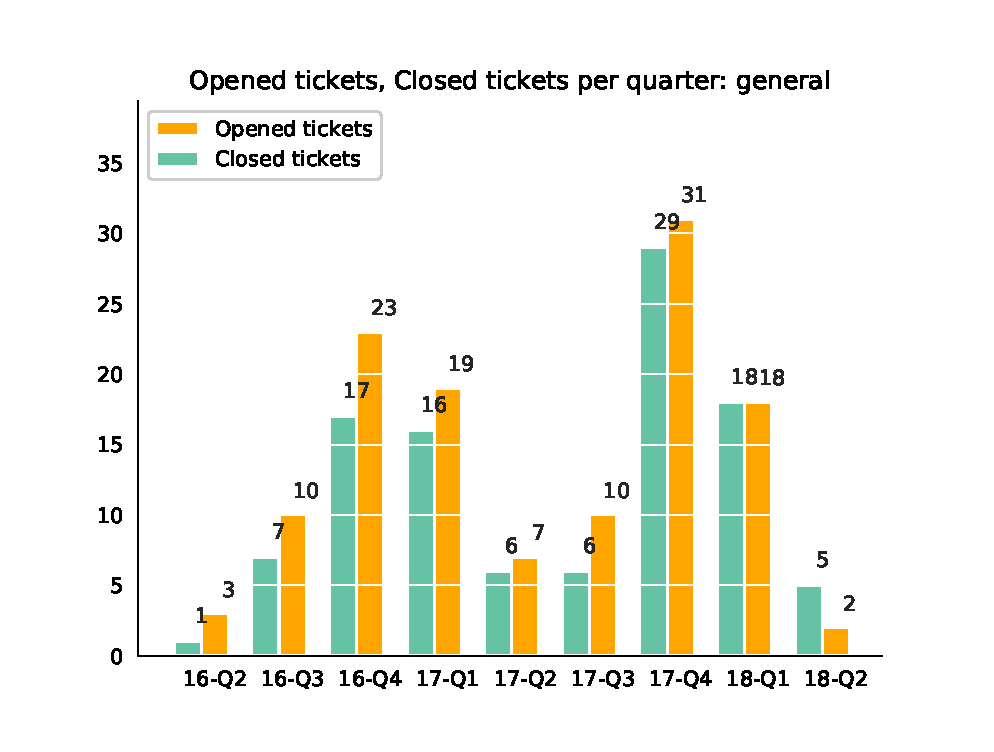
\includegraphics[scale=.75]{activity/github_issues_opened_github_issues_closed.eps}
	& 
	\vspace{0pt}
	\begin{tabular}{l|r|r|}%
		\bfseries Period & \bfseries Opened & \bfseries Closed % specify table head
		\csvreader[head to column names]{activity/github_issues_opened_github_issues_closed.csv}{}% use head of csv as column names
		{\\\Date & \opened & \closed}
	\end{tabular}
\end{tabular}